
\documentclass{article}
\usepackage[utf8]{inputenc}
\usepackage[english]{babel}
\usepackage{amsmath}
\usepackage{amsthm} 
\usepackage{amssymb}
\usepackage{tikz}
\usetikzlibrary{positioning, arrows.meta, calc}
\usepackage[most]{tcolorbox}
\usepackage{xcolor,tcolorbox}
\usepackage{geometry}
\usepackage{graphicx}
\usepackage{longtable}
\usepackage{tabularx}
\usepackage{booktabs}
% Настройка теорем и других математических элементов


\title{Will: A Unified Framework\\
PART I - RELATIVITY'S}
\author{Anton Rize egeometricity@gmail.com}
\date{April 2025}

% Пакеты
\usepackage[utf8]{inputenc}        % Кодировка
\usepackage[T2A]{fontenc}          % Кодировка шрифтов
\usepackage[english]{babel} % Языки                             
\usepackage{graphicx} 

% Настройки полей страницы
\geometry{
    a4paper,
    left=25mm,
    right=25mm,
    top=25mm,
    bottom=25mm,
}

% Новые команды для модели
\newcommand{\QGModel}{QG model}

\begin{document}
\theoremstyle{definition}
\newtheorem{definition}{Definition}
\newtheorem{theorem}{Theorem}
\newtheorem{lemma}{Lemma}
\newtheorem{corollary}{Corollary}

\maketitle

\begin{figure}[!htb]
    \centering
    \includegraphics[width=0.75\linewidth]{img/IMG.jpg}
    \caption{$\kappa$, $\beta$  and orthogonal reflections $T_c$, $L_c$ as Energy projections on unit circle r = c }
\end{figure}

\newpage

\tableofcontents

\section{Will: A Relational Framework for Space-Time-Energy}

\subsection{Motivation and Core Principles}

The standard formulation of General Relativity often relies on the concept of an asymptotically flat spacetime, introducing an implicit external reference frame beyond the physical systems under study. While some modern approaches (e.g., shape dynamics) seek greater relationality, we proceed from strict epistemic minimalism, disallowing all background structures, even hidden or asymptotic ones.

\textbf{Principle:} \emph{All physical quantities must be defined purely by their relations.} Any introduction of absolute properties or external frames risks reintroducing metaphysical artifacts and contradicts the foundational insight of relativity.

\vspace{1em}
\textbf{What is Energy?} Energy is not an intrinsic property of objects, but a measure of difference between possible states. It expresses the system's capacity to transition, always encountered as a relative potential for change—not as something possessed, but as a comparative structure between observers. In this framework, energy marks the directional tendency for one configuration to transform into another.

\vspace{1em}
We therefore posit a single unifying axiom:

\begin{center}
\boxed{\text{SPACETIME} \equiv \text{ENERGY EVOLUTION}}
\end{center}

\textbf{Clarification:} By ``energy evolution'' we mean the total structure of possible transitions between observable states---not a process unfolding in spacetime, but the very relational geometry from which both space and time emerge. This is not a derived result, but a foundational postulate, subject to geometric and empirical audit in subsequent sections. ``Will'' is used here as a technical term for this unified, emergent structure.


\subsection{Fundamental Structure of Will}

From our postulate, several key properties of the Will framework can be derived:

\begin{enumerate}
    \item \textbf{Self-contained geometry:} Since spacetime is identical to energy evolution, there can be no external objects or reference frames. The geometry must therefore be self-contained.
    
    \item \textbf{Conservation law:} A closed geometry naturally leads to conservation principles—nothing enters or leaves the system, making the total energy constant.
    
    \item \textbf{Symmetry:} With no external reference, all directions/positions must be equivalent; any asymmetry would require a preferred frame, which is disallowed. 
    
    \item \textbf{Circular geometry:} Among all closed and maximally symmetric geometries, the circle (and, in higher dimensions, the sphere) uniquely preserves equivalence of all points and directions, ensuring that no hidden reference structure or asymmetry contaminates the framework.
\end{enumerate}

\subsection{Emergence of Space and Time}
\textit{In this construction, space and time are not assumed as independent entities, but arise as complementary projections of the underlying rate and direction of energetic transformation along the closed geometric structure.}

The word "evolution" in our postulate implies a non-instantaneous process, requiring a rate of change. This rate naturally establishes a relationship between what we perceive as spatial and temporal units, yielding the speed of evolution.

Any energy state can be represented as a point on the circle. Changes in energy states correspond to movement along this circle, characterized by:
\begin{itemize}
    \item Speed of state change (rate of evolution)
    \item Direction of state change
\end{itemize}

These two orthogonal components naturally give rise to what we interpret as space-like and time-like dimensions without needing to postulate coordinate axes a priori.

\subsection{Fundamental Theorem of Will}
\textit{In this view, the Will manifold encodes all physically meaningful structure as patterns of relational evolution, with no background space, and local features such as causality and intensity emerging solely from the intrinsic properties of this flow.}

\begin{theorem}[Structure of Will Manifold]
The Will manifold $\mathcal{W}$ is defined as the space of all possible energy relations between systems, such that:
\begin{enumerate}
    \item For any two systems $S_1$ and $S_2$, there exists an energy relation $E(S_1, S_2) \in \mathcal{W}$
    \item The evolution of energy relations defines a flow on $\mathcal{W}$
    \item This flow induces a circular topology on $\mathcal{W}$ where continuity is defined by continuous energy transformations
    \item The causal structure emerges from the directional properties of this flow
    \item The local structure of $\mathcal{W}$ is determined by the intensity of energy relations


\end{enumerate}

\begin{proof}

\section{Mathematical Foundation}

\subsection{Reinterpretation of speed of light:}

We interpreting the \textbf{speed of light} $\textbf{c}$ as the \textbf{universal rate of change} implying that every energy transformation or interaction has the same rate = c distributed  between spatial like and temporal like components. We expressing \textbf{universal rate of change}\textbf{ c} as rotating radial vector so the unit circle naturally emerges as embodiment of conservation law:

\begin{itemize}
    \item \textbf{$r=c = 1$} rotating radial vector on a unit circle controlled by:
    \item \textbf{$\theta_S = \arccos(\beta)$} relativistic angle represents energy distribution by rotation of radial vector.
\end{itemize}
\begin{itemize}
    \item  \textbf{$ \beta =  \frac{v}{c} = \sqrt{\frac{R_s}{2r}} =  \cos\left(\theta_S\right), \quad \text{(Orbital velocity)}$} space like kinetic component ($X$axis) 
\end{itemize}
    \begin{itemize}
        \item   $L_c =\sqrt{1-\beta^2} =\sin(\theta_S)\text{ (Length contraction factor)}$ temporal like component  ($Y$axis) 
        \item $T_d =\frac{1}{L_c}=\frac{1}{\sqrt{1-\beta^2} }=\frac{1}{\sin(\theta_S)}\text{ (Time dilation factor)}$ identical to relativistic $\gamma$ factor.
    \end{itemize}

In our model, the spatial and temporal-like projections are not to be interpreted as traditional coordinates, but as relative geometric ratios derived from the invariant rate of change. 

\subsubsection{Special Theory of Relativity (Time Dilation Factor)}

The standard time dilation factor in Special Relativity is given by:
\begin{equation}
T_d = \frac{1}{\sqrt{1 - \frac{v^2}{c^2}}}.
\end{equation}

Our geometric expression for the relativistic factor is:
\begin{equation}
T_d = \frac{1}{\sin(\arccos(\beta))},
\end{equation}
where:
\begin{equation}
\beta = \frac{v}{c}.
\end{equation}
\textbf{Derivation of Equivalence:}
1. Start with the geometric expression:
\begin{equation}
T_d = \frac{1}{\sin(\arccos(\beta))}.
\end{equation}

2. Use the trigonometric identity \(\sin^2(x) + \cos^2(x) = 1\), which implies \(\sin(x) = \sqrt{1 - \cos^2(x)}\):
\begin{equation}
T_d = \frac{1}{\sqrt{1 - \cos^2(\arccos(\beta))}}.
\end{equation}

3. Evaluate \(\cos(\arccos(\beta))\):
\begin{equation}
T_d = \frac{1}{\sqrt{1 - \beta^2}}= \frac{1}{\sqrt{1 - \frac{v^2}{c^2}}}=\gamma.
\end{equation}
\textbf{Conclusion:} The derived expression is identical to the standard time dilation factor, demonstrating the equivalence.

\subsection{Interpretation of \(\beta\): Spatial Energy Projection}

$\beta$ quantifies the energy of an object or system as expressed in terms of the relative rate of change of spatial coordinates. Operationally, it reflects the amount of energy the observer would need to expend to "catch up" with the object.

The range of \(\beta\) is naturally constrained:
\[
0 \leq \beta \leq 1
\]
Beyond \(\beta = 1\), the object moves faster than the speed at which causal signals propagate (speed of light in vacuum), and therefore becomes causally disconnected from the observer.

\subsection{Derivation of Energy-Momentum Relation and $E=mc^2$}

Having established the geometric interpretation of relativistic effects through the unit circle, we can now derive the fundamental energy-momentum relation and Einstein's famous equation $E=mc^2$ directly from our Will framework.

\subsubsection{Energy as a Vector in Will Geometry}

In our model, we interpret energy as a vector on the $(X,Y)$ plane:
\begin{itemize}
    \item The vector's length (hypotenuse) equals $c$ for a given mass $m$
    \item The vector's orientation is determined by the relativistic angle $\theta_S$
    \item The distribution between spatial and temporal components is governed by this angle
\end{itemize}

\subsubsection{Geometric Components of the Energy Vector}

For an object with mass $m$, the components of the energy vector are:
\begin{align}
    \text{Spatial component (X-axis):} & \quad c \cdot \cos(\theta_S) = c \cdot \beta \\
    \text{Temporal component (Y-axis):} & \quad c \cdot \sin(\theta_S) = c \cdot \sqrt{1-\beta^2}
\end{align}

The ratio of these components is given by:
\begin{equation}
    \cot(\theta_S) = \frac{\beta}{\sqrt{1-\beta^2}} = \beta \cdot \gamma
\end{equation}

\subsubsection{Definition of Momentum and Energy}

For an object with mass $m$:
\begin{align}
    \text{Momentum } p &= m \cdot \beta \cdot \gamma \cdot c = \gamma m v \\
    \text{Temporal energy component } E_t &= m \cdot \gamma \cdot c^2
\end{align}

These definitions emerge naturally from the geometric projections and do not rely on prior knowledge of relativistic formulas.

\subsubsection{Derivation of the Energy-Momentum Relation}

The total energy vector has a squared magnitude:
\begin{align}
    E^2 &= (m \cdot \gamma \cdot c^2)^2 + (p \cdot c)^2 \\
\end{align}

Substituting $p = \gamma m v = \gamma m \cdot c \cdot \beta$:
\begin{align}
    E^2 &= (m \cdot \gamma \cdot c^2)^2 + (\gamma \cdot m \cdot c \cdot \beta \cdot c)^2 \\
    &= \gamma^2 m^2 c^4 + \gamma^2 m^2 c^2 \cdot \beta^2 c^2 \\
    &= \gamma^2 m^2 c^4(1 + \beta^2)
\end{align}
\begin{align}
    E^2 &= \gamma^2 m^2 c^4(1 + \beta^2) \\
\end{align}
Since $\gamma^2 = \frac{1}{1-\beta^2}$:
\begin{align}
    E^2 &= m^2 c^4 \cdot \frac{1 + \beta^2}{1-\beta^2} \\
    &= m^2 c^4 \cdot \frac{1}{1-\beta^2} + m^2 c^4 \cdot \frac{\beta^2}{1-\beta^2} \\
\end{align}

Given that $p^2 = \gamma^2 m^2 v^2 = \gamma^2 m^2 c^2 \beta^2 = \frac{m^2 c^2 \beta^2}{1-\beta^2}$:
\begin{align}
    E^2 &= m^2 c^4 + p^2 c^2 \\
\end{align}

Simplifying:
\begin{equation}
    \boxed{E^2 = m^2 c^4 + p^2 c^2}
\end{equation}
For an object at rest ($\beta = 0, p = 0$):
\begin{equation}
    \boxed{E_0 = mc^2}
\end{equation}

\subsubsection{Geometric Interpretation}

The derivation reveals that Einstein's famous equation $E=mc^2$ and the relativistic energy-momentum relation emerge directly from the Pythagorean theorem applied to our energy vector on the Will unit circle. The $c^2$ term arises naturally as the square of the hypotenuse (radius), not as an arbitrary dimensional factor.

This geometric approach unifies our understanding of mass, energy, and momentum as different projections of the same fundamental quantity—the energy vector in Will geometry—whose orientation is determined by the relative motion between observer and observed system.

\section{Gravitational Extension}

\subsection{Conceptual Foundation}

\subsubsection{Beyond Curvature: A New Perspective}

The conventional approach to gravity in General Relativity relies on the concept of curvature—a notion that implicitly assumes the existence of a flat reference frame. This creates a fundamental inconsistency: while rejecting absolute space in principle, standard GR tacitly introduces an absolute reference through the concept of curvature relative to flatness.

In our Will framework, we reject this artifice. Rather than imposing curvature as an interpretational construct, we allow the universe to naturally manifest its geometric structure through energy relations. This approach remains true to our foundational principle:

\begin{center}
\boxed{\text{SPACETIME} \equiv \text{ENERGY EVOLUTION}}
\end{center}

\subsubsection{Dimensional Analysis of Gravitational Energy}

If gravity operates within the same geometric structure as relativistic velocity, we must express it as a dimensionless fraction of the speed of light, since we operate on a circle with radius $c$. However, gravity and velocity differ in their dimensional characteristics:

\begin{itemize}
    \item $\beta$ represents one-dimensional energy distribution as a motion vector (1D): $\frac{v}{c}$
    \item Gravity represents three-dimensional energy distribution as an isotropic field with $\frac{1}{r}$ dependence
\end{itemize}

This distinction leads us to introduce a new parameter $\kappa$ to characterize gravitational energy distribution. While $\beta$ represents a directional (vector) quantity, $\kappa$ represents a radial (scalar) quantity distributed across a spherical surface (2D).

\subsubsection{Boundary Conditions and Physical Interpretation}

For kinetic energy parameter $\beta$:
\begin{itemize}
    \item $\beta = 0$: No relative motion
    \item $\beta = 1$: Maximum possible relative motion (speed of light)
\end{itemize}

By analogy, for the gravitational parameter $\kappa$:
\begin{itemize}
    \item $\kappa = 0$: No gravitational influence
    \item $\kappa = 1$: Maximum possible gravitational influence (event horizon)
\end{itemize}

The value $\kappa = 1$ corresponds precisely to the point where escape velocity equals the speed of light, creating an event horizon. This provides a natural upper bound for our gravitational parameter, analogous to the light-speed limit for relative motion.

The striking parallel between these parameters suggests a profound geometric connection between kinetic and potential energy within the Will framework, which we shall now formalize mathematically:

Equivalent to our previous derivation of $\beta$ as kinetic energy component, now we can derive $\kappa$:
\begin{itemize}
    \item  \textbf{$ \kappa =  \frac{v_e}{c} = \sqrt{\frac{R_s}{r}} =  \sin\left(\theta_G\right), \quad \text{(Escape velocity)}$}. time like potential component ($Y$axis) 
\end{itemize}
\begin{itemize}
    \item \textbf{$\theta_G = \arcsin(\kappa)$} gravitational angle represents potential energy distribution.
\end{itemize}
    \begin{itemize}
        \item   $T_c =\sqrt{1-\kappa^2}=\sqrt{1-\frac{R_s}{r}}  =\cos(\theta_G)\text{ (Time contraction factor)}$ spatial like component  ($X$axis) 
        \item $L_d =\frac{1}{T_c}=\frac{1}{\sqrt{1-\kappa^2} }=\frac{1}{\cos(\theta_G)}\text{ (Length dilation factor)}$.
    \end{itemize}
where $R_s = \frac{2GM}{c^2}$
\subsubsection{General Theory of Relativity (Length Dilation Factor)}
The relevant component of the Schwarzschild metric, related to gravitational length dilation, is given by:
\begin{equation}
L_d = \frac{1}{\sqrt{1 - \frac{2GM}{rc^2}}} = \frac{1}{\sqrt{1 - \frac{R_s}{r}}}.
\end{equation}
Our geometric expression for the gravitational factor is:
\begin{equation}
L_d = \frac{1}{\cos(\arcsin(\kappa))},
\end{equation}
where:
\begin{equation}
\kappa^2 = \frac{R_s}{r}.
\end{equation}
\textbf{Derivation of Equivalence:}
1. Start with the geometric expression:
\begin{equation}
L_d = \frac{1}{\cos(\arcsin(\kappa))}.
\end{equation}
2. Use the trigonometric identity \(\cos(x) = \sqrt{1 - \sin^2(x)}\):
\begin{equation}
L_d = \frac{1}{\sqrt{1 - \sin^2(\arcsin(\kappa))}}.
\end{equation}
3. Evaluate \(\cos(\arcsin(\kappa))\):
\begin{equation}
L_d = \frac{1}{\sqrt{1 - \kappa^2}}=
\frac{1}{\sqrt{1 - \frac{R_s}{r}}}.
\end{equation}
\textbf{Conclusion:} The derived expression is identical to the relevant component of the Schwarzschild metric, demonstrating the equivalence.

\subsubsection{Interpretation of \(\kappa\): Temporal Energy Projection}
This parameter quantifies the energy content of the object expressed through the relative rate of change of temporal coordinates. It characterizes how much energy the object would need to "escape" its local temporal curvature and synchronize its temporal coordinates with the observer.

\subsubsection{Unified Interpretation}
 \(\beta\) and \(\kappa\) represent dimensionless measures of the energy distribution of an object or system, expressed through its relative projection onto spatial and temporal aspects of the observer's reference frame.
Together, they describe the energetic structure of causality in the observer's reference frame:
\begin{itemize}
    \item \(\beta\) governs local, kinematic accessibility (relative spatial motion).
    \item \(\kappa\) governs global, potential accessibility (relative temporal displacement).
\end{itemize}
These parameters form the basis of the energy-geometric interpretation of spacetime structure, where space, time, and energy are unified as projections of a single underlying geometric entity Will.

\subsection{Fundamental Relation Between Gravitational and Kinetic Energy Parameters}

\subsubsection{The Principle of Unified Energy Budget}

According to our foundational postulate, $\text{SPACETIME} \equiv \text{ENERGY EVOLUTION}$, both $\kappa$ and $\beta$ represent different projections of the same underlying energy evolution. This implies a strict conservation principle: the total energy budget must be distributed between these parameters according to a fundamental ratio.

\subsubsection{Geometric Derivation from First Principles}

To derive the precise relationship between $\kappa$ and $\beta$ from purely geometric considerations:

\begin{enumerate}
    \item We know that $\beta$ represents a one-dimensional distribution of energy (directional vector).
    \item We know that $\kappa$ represents a two-dimensional distribution of energy (spherically symmetric field through $1/r$ dependence).
    \item Both parameters are normalized dimensionless ratios relative to the speed of light $c$.
\end{enumerate}

In a perfectly symmetric, closed geometric system, the maximum extent of energy distribution for each parameter is determined by the geometry of the parameter's dimensionality:

\begin{itemize}
    \item For $\beta$ (1D parameter): Maximum symmetric distribution = circumference of unit circle = $2\pi$
    \item For $\kappa$ (2D parameter): Maximum symmetric distribution = surface area of unit sphere = $4\pi$
\end{itemize}

The ratio of these maximum distributions yields:
\begin{equation}
\frac{4\pi}{2\pi} = 2
\end{equation}

This represents the fundamental geometric ratio between the two-dimensional and one-dimensional projections of energy in our model.

\subsubsection{Degrees of Freedom Analysis}

This same ratio emerges when analyzing the degrees of freedom for energy distribution:
\begin{itemize}
    \item $\beta$ has 1 degree of freedom (direction along a line)
    \item $\kappa$ has 2 degrees of freedom (distribution across a spherical surface)
\end{itemize}

The ratio of available geometric space for energy distribution is thus 2:1.

\subsubsection{Fundamental Conservation Law}

This leads us to the fundamental relation:

\begin{equation}
\boxed{\frac{\kappa^2}{\beta^2} = 2}
\end{equation}

This equation represents a profound geometric conservation principle that governs the distribution of energy between gravitational (potential) and kinetic aspects before the emergence of spacetime itself.

\subsubsection{Universal Significance}

While this relation can be derived in specific contexts like orbital mechanics, such derivations merely reflect the manifestation of this deeper geometric principle in particular physical scenarios. Our derivation proceeds solely from the symmetry and closure requirements of the Will framework, without introducing any additional assumptions or physical laws.

This relation is not a consequence of physics—rather, physics is a consequence of this fundamental geometric relationship between energy projections.

\subsection{Geometric Relationships}

The relativistic and gravitational factors can be expressed in unified algebraic and trigonometric forms, as shown in Table 1.

\begin{table}[h]
\centering
\begin{tabular}{|c|c|}
\hline
\textbf{Algebraic Form} & \textbf{Trigonometric Form} \\
\hline
$T_d = \frac{1}{\sqrt{1-\beta^2}}$ & $T_d = \frac{1}{\sin(\theta_S)} = \frac{1}{\sin(\arccos(\beta))}$ \\
\hline
$L_d = \frac{1}{\sqrt{1-\kappa^2}}$ & $L_d = \frac{1}{\cos(\theta_G)} = \frac{1}{\cos(\arcsin(\kappa))}$ \\
\hline
$L_c = \sqrt{1-\beta^2}$ & $L_c = \sin(\theta_S) = \sin(\arccos(\beta))$ \\
\hline
$T_c = \sqrt{1-\kappa^2}$ & $T_c = \cos(\theta_G) = \cos(\arcsin(\kappa))$ \\
\hline
\end{tabular}
\caption{Unified representation of relativistic and gravitational effects.}
\end{table}

\subsubsection{The Combined Energy Parameter $Q$}

The total energy projection parameter unifies both aspects:

\begin{align}
    Q &=\sqrt{\kappa^2 + \beta^2}  \\
    Q^{2}&= 3\beta^2 = \frac{3}{2}\kappa^2 = \frac{3R_s}{2r_{dis}} \\
    Q_t &= \sqrt{1-Q^2} = \sqrt{1-\kappa^2-\beta^2} = \sqrt{1-3\beta^2} = \sqrt{1-\frac{3}{2}\kappa^2} \\
    Q_r &= \frac{1}{Q_t}
\end{align}

These describe the combined effects of relativity and gravity.

\begin{tcolorbox}[colback=gray!5, colframe=black!80!black, title=Unified Interpretation]
Our geometric approach is mathematically equivalent to the standard formulas but reveals their unified origin. It demonstrates that relativistic and gravitational effects emerge from the same geometric principles, represented by the parameters $\beta$ and $\kappa$.
\end{tcolorbox}


\subsection{Energy Reciprocity Law}

\subsubsection{Causal Continuity and the Energy Reciprocity Law}

\begin{theorem}[Energy Reciprocity]
The energy differences perceived by two observers at different positions are balanced according to the Energy Reciprocity Law:
\begin{align}
\Delta E_{\text{A}\rightarrow\text{B}} + \Delta E_{\text{B}\rightarrow\text{A}} = 0.
\end{align}
\end{theorem}

\begin{proof}
Consider an astronomer on the surface of a planet at radius $r_A = R_{\text{planet}}$ and a cosmonaut in a stable circular orbit at radius $r_C = r_{\text{orbit}} > r_A$.

From the astronomer's perspective:
\begin{itemize}
\item The cosmonaut is at a higher gravitational potential and moves with orbital speed.
\item To match the cosmonaut's state, the astronomer must escape from $r_A$ to $r_C$ and acquire the orbital speed.
\item This requires gaining energy, described by
\begin{align}
\Delta E_{\text{astronomer}\rightarrow\text{cosmonaut}} = (\kappa^2_A - \kappa^2_C) + \beta^2_C.
\end{align}
\end{itemize}

From the cosmonaut's perspective:
\begin{itemize}
\item The astronomer is deeper in the gravitational well and at rest.
\item To synchronize with the astronomer, the cosmonaut must descend to $r_A$ and lose kinetic energy.
\item This requires losing energy, described by
\begin{align}
\Delta E_{\text{cosmonaut}\rightarrow\text{astronomer}} = (\kappa^2_C - \kappa^2_A) - \beta^2_C.
\end{align}
\end{itemize}

Each observer perceives the energy difference through complementary parameters, reflecting the observer-centered nature of Will Geometry.

The energy differences are balanced according to the Energy Reciprocity Law:
\begin{align}
\Delta E_{\text{astronomer}\rightarrow\text{cosmonaut}} + \Delta E_{\text{cosmonaut}\rightarrow\text{astronomer}} = 0.
\end{align}

With:
\begin{align}
\Delta E_{\text{astronomer}\rightarrow\text{cosmonaut}} &= (\kappa^2_A - \kappa^2_C) + \beta^2_C, \\
\Delta E_{\text{cosmonaut}\rightarrow\text{astronomer}} &= (\kappa^2_C - \kappa^2_A) - \beta^2_C,
\end{align}
where
\begin{align}
\kappa^2_A = \frac{R_s}{r_A}, \kappa^2_C = \frac{R_s}{r_C}, \beta^2_C = \frac{R_s}{2r_C}, R_s = \frac{2GM}{c^2}.
\end{align}

Summing the two:
\begin{align}
\Delta E_{\text{astronomer}\rightarrow\text{cosmonaut}} + \Delta E_{\text{cosmonaut}\rightarrow\text{astronomer}} &= [(\kappa^2_A - \kappa^2_C) + \beta^2_C] + [(\kappa^2_C - \kappa^2_A) - \beta^2_C] \\
&= (\kappa^2_A - \kappa^2_A) + (-\kappa^2_C + \kappa^2_C) + (\beta^2_C - \beta^2_C) \\
&= 0
\end{align}

Thus, the total energy exchange balances exactly, confirming the Energy Reciprocity Law. This law ensures that the total energetic difference between observers sums to zero, preserving causality and consistency.

\subsubsection{Observer-Agnostic Reciprocity for Arbitrary Energy Functions}

The reciprocity principle between two observers does not depend on the specific geometric or metric model of motion, but only on the symmetry of energy difference perception.

Let the cosmonaut be in an arbitrary orbital or dynamic state with energy characterized by some function \( f(v) \), where \( v \) is the local velocity of the cosmonaut as perceived by an external observer. The exact form of \( f \) is irrelevant—it can follow Newtonian, relativistic, or any other framework—as long as both observers agree on its operational meaning.

From the astronomer's perspective:
\begin{itemize}
    \item The cosmonaut is at a different gravitational potential and possesses motion described by \( f(v) \).
    \item To match the cosmonaut's state, the astronomer must gain energy:
    \[
    \Delta E_{A \rightarrow C} = \Delta \Phi + f(v),
    \]
    where \( \Delta \Phi \) represents the gravitational potential difference.
\end{itemize}

From the cosmonaut's perspective:
\begin{itemize}
    \item The astronomer lies deeper in the potential well and has no kinetic component.
    \item To match the astronomer's state, the cosmonaut must lose energy:
    \[
    \Delta E_{C \rightarrow A} = -\Delta \Phi - f(v).
    \]
\end{itemize}

Summing both expressions yields:
\[
\Delta E_{A \rightarrow C} + \Delta E_{C \rightarrow A} = (\Delta \Phi + f(v)) + (-\Delta \Phi - f(v)) = 0.
\]

\begin{tcolorbox}[colback=gray!5, colframe=black!80!black, title=Geometric Independence]
This demonstrates that the Energy Reciprocity Law holds for any energy function \( f(v) \), regardless of the geometry, orbit type, or spacetime metric. For any two observers A and C in any potential or dynamical context: 
\[
\boxed{
\Delta E_{A \rightarrow C} + \Delta E_{C \rightarrow A} = 0 \quad \forall \ f(v)
}
\]
What matters is not how energy is geometrically expressed, but that observers agree on its differential accounting.
\end{tcolorbox}

\[
\boxed{

\Delta E_{A\rightarrow C} + \Delta E_{C\rightarrow A} = 0 \implies \text{Energy is redistributed, never created nor lost.}}

\]
\end{proof}

\subsection{Why the Speed of Light Cannot Be Exceeded}

\begin{theorem}[Universal Speed Limit]
The universal speed limit emerges naturally from the structure of Will Geometry.
\end{theorem}

\begin{proof}
Let us consider the spatial projection parameter $\beta = \frac{v}{c}$, and the temporal projection parameter $\kappa = \sqrt{\frac{R_s}{r}}$. These represent, respectively, the kinetic and gravitational energy components of an observer-object system, expressed as dimensionless projections on orthogonal axes.

If an object were to exceed the speed of light, then:
\begin{align}
\beta > 1 \Rightarrow \beta^2 > 1
\end{align}

Since $\kappa^2 \leq 1$ for all physically realizable positions ($r \geq R_s$), it follows that:
\begin{align}
\Delta E_{\text{observer}} = \beta^2 - \kappa^2 > 1 - \kappa^2 > 0
\end{align}

This results in an unbalanced energy difference that cannot be reciprocated from the object's frame:
\begin{align}
\Delta E_{\text{observer}} + \Delta E_{\text{object}} \neq 0
\end{align}
which violates the Energy Reciprocity Law. The energy structure becomes asymmetric, breaking the internal balance required for causal consistency.

Therefore, the condition $\beta \leq 1$ is not imposed externally but arises as a necessary consequence of maintaining energetic symmetry and causal continuity between observers. Beyond the limit $\beta \leq 1$, the observer-object energetic system becomes unbalanced, making reciprocal synchronization of causal states impossible. The speed of light limit ensures that no observer ever perceives a net gain or loss of energy without cause.

In essence, Will Geometry encodes the principle that:
\begin{quote}
The speed of light is the boundary beyond which the energetic symmetry between perspectives breaks down. Causality is not an external rule but a built-in feature of the universe's energetic geometry.
\end{quote}
\end{proof}


\section{Derivation of Energy Density, Pressure and Mass Relations from Geometric First Principles}

In this section, we derive the expressions for the local energy density $\rho(r_{\text{dis}})$, the critical energy density $\rho_{\text{max}}$, and the enclosed mass $m_0$ purely within the geometric framework based on first principles. The derivation relies only on the spherical symmetry of energy distribution and the geometric parameter $\kappa$, which encodes the local curvature through energy content.

\subsubsection{Geometric Foundation}

We define the curvature parameter $\kappa$ as:
\begin{equation}
\kappa^2 = \frac{R_s}{r_{\text{dis}}} = \frac{2G m_0}{c^2 r_{\text{dis}}},
\end{equation}
where $R_s$ is the Schwarzschild radius associated with the enclosed mass $m_0$. This relation is purely geometric and follows from the spherical symmetry of energy distribution.

\subsubsection{Expression for Enclosed Mass}

From the definition of $\kappa^2$, the enclosed mass within radius $r_{\text{dis}}$ is:
\begin{equation}
m_0 = \frac{c^2}{2G} \kappa^2 r_{\text{dis}}.
\end{equation}
\subsubsection{Geometric Definition of Energy Density}

By the geometric definition of mass in terms of local energy density:
\begin{equation}
\frac{d m_0}{d r_{\text{dis}}} = 4\pi r_{\text{dis}}^2 \rho(r_{\text{dis}}),
\end{equation}
and substituting the expression for $m_0$:
\begin{equation}
\frac{d}{d r_{\text{dis}}} \left( \kappa^2 r_{\text{dis}} \right) = \frac{8\pi G}{c^2} r_{\text{dis}}^2 \rho(r_{\text{dis}}).
\label{eq:geo_density}
\end{equation}
This equation is a purely geometric identity linking the radial variation of the curvature parameter $\kappa$ to the local energy density.

\subsubsection{Stationary Case and Critical Density}

In the case of a stationary, spherically symmetric system with constant $\kappa$, the derivative simplifies:
\begin{equation}
\frac{d}{d r_{\text{dis}}} \left( \kappa^2 r_{\text{dis}} \right) = \kappa^2.
\end{equation}
Equation (\ref{eq:geo_density}) then yields:
\begin{equation}
\kappa^2 = \frac{8\pi G}{c^2} r_{\text{dis}}^2 \rho(r_{\text{dis}}).
\end{equation}
Solving for $\rho(r_{\text{dis}})$:
\begin{equation}
\rho(r_{\text{dis}}) = \frac{\kappa^2 c^2}{8\pi G r_{\text{dis}}^2}.
\end{equation}
We define the \textbf{local critical energy density} as the maximum achievable density at which the entire curvature parameter is realized by the local energy content:
\begin{equation}
\kappa = 1 \quad \Rightarrow \quad \rho_{\text{max}} = \frac{c^2}{8\pi G r_{\text{dis}}^2}.
\end{equation}
\subsubsection{Physical Interpretation of Critical Density}

The condition $\kappa = 1$ corresponds to the situation where the local curvature induced by energy density reaches the Schwarzschild limit:
\begin{equation}
R_s = r_{\text{dis}}.
\end{equation}
This defines the formation of an event horizon and the onset of gravitational collapse. Beyond this point, any further increase in energy density does not affect the external geometry — it is hidden behind the horizon. Therefore, $\rho_{\text{max}}$ represents the \textbf{maximum locally measurable energy density} within the observable universe.

Higher values of $\kappa$ (\(\kappa > 1\)) may appear in rotating systems (e.g., Kerr metric) as a result of global redistribution of energy and angular momentum but do not correspond to locally accessible densities.

\subsubsection{Mass Expression}

Integrating the energy density over a sphere of radius $r_{\text{dis}}$, the enclosed mass is:
\[
m_0(r_{\text{dis}}) = \int_0^{r_{\text{dis}}} 4\pi r'^2 \rho(r') \, d r' 
\quad \Longrightarrow \quad m_0(r_{\text{dis}}) = \frac{c^2}{2G} \kappa^2 r_{\text{dis}}.
\]

This confirms the internal consistency of the model, where the energy content and geometric curvature are directly and uniquely related.

\begin{tcolorbox}[colback=gray!5,colframe=black!40!black,title=Epistemological Note]
The derivation above introduces no postulated spacetime manifold, coordinates, or metric tensors. All expressions arise directly from the observer-relative energetic geometry encoded in the projection parameter $\kappa$. Mass and density are not assumed but defined as emergent quantities consistent with the energetic curvature of space as perceived by an observer at radius $r_{\text{dis}}$.
\end{tcolorbox}



\begin{tcolorbox}[colback=gray!4, colframe=black!80!black, title=Foundational Clarification]
This model does not impose surface-based energy projection as a postulate.\\
Instead, it derives it from the dimensional symmetry of projection:
\[
\boxed{\kappa^2 = 2 \beta^2}
\quad \Rightarrow \quad
\frac{\text{Area}(S^2)}{\text{Length}(S^1)} = 2.
\]
This ratio naturally defines the curvature-based energy projection over spherical boundaries, with no need to assume volumetric content.\\

Thus, mass and pressure emerge as functions of surface curvature, not as integrations over filled 3D volume.\\
Volume is a derived artifact — surface is primary.
\end{tcolorbox}

\subsection{Pressure as Surface Curvature Gradient}

Pressure in Will Geometry emerges directly from the gradient of curvature:
\begin{align}
P(r_{dis}) = - \frac{c^2}{8\pi G} \cdot \frac{1}{r_{dis}} \cdot \frac{d\kappa^2}{dr_{dis}}
\end{align}
Consider the relationship between pressure and energy gradient. In a spherically symmetric system in hydrostatic equilibrium, the pressure gradient must compensate for changes in the system's energy state.

Since $\kappa^2$ represents a normalized energy parameter related to gravitational potential:
\begin{align}
\kappa^2 = \frac{R_s}{r_{\text{dis}}} = \frac{2Gm_0}{c^2 r_{\text{dis}}}
\end{align}
The change of this parameter with radius, $\frac{d\kappa^2}{dr_{\text{dis}}}$, reflects the gradient of potential energy. To maintain energy balance, this change must be related to the pressure gradient.

Since pressure is a measure of energy per unit volume, and given that energy density is related to $\kappa^2$ through:
\begin{align}
\rho(r_{\text{dis}}) = \frac{\kappa^2 c^2}{8\pi G r_{\text{dis}}^2}
\end{align}
It can be shown that the pressure gradient must satisfy:
\begin{align}
P(r_{\text{dis}}) = - \frac{c^2}{8\pi G} \cdot \frac{1}{r_{\text{dis}}} \cdot \frac{d\kappa^2}{dr_{\text{dis}}}
\end{align}
This expression establishes a direct link between pressure and changes in curvature, without the need to postulate an internal volume structure.

\begin{center}
\boxed{\text{The Universe is not embedded in geometry; geometry emerges from energy.}}
\end{center}

\subsection{Unified Geometric Field Equation}

\subsubsection{Derivation of the Field Equation}

\begin{theorem}[Geometric Field Equation]
The relationship between curvature and energy density follows:
\begin{align}
\frac{d}{dr_{\text{dis}}}(\kappa^2 \cdot r_{\text{dis}}) = \frac{8\pi G}{c^2}r_{\text{dis}}^2 \cdot \rho(r_{\text{dis}})
\end{align}
\end{theorem}

\begin{proof}
Starting with the mass enclosed within radius $r_{\text{dis}}$:
\begin{align}
M(r_{\text{dis}}) = \int_0^{r_{\text{dis}}} 4\pi r'^2 \rho(r')dr'
\end{align}


$Z_{\rm eff}^{(0)}(r)
=Z-\int_0^r \rho_{\rm el}^{(0)}(r')4\pi r'^2dr$
The corresponding Schwarzschild radius is:
\begin{align}
R_s(r_{\text{dis}}) = \frac{2GM(r_{\text{dis}})}{c^2}
\end{align}
Since $\kappa^2 = \frac{R_s(r_{\text{dis}})}{r_{\text{dis}}}$, it follows that:
\begin{align}
\kappa^2 r_{\text{dis}} = R_s(r_{\text{dis}})
\end{align}
Differentiating both sides with respect to $r_{\text{dis}}$:
\begin{align}
\frac{d}{dr_{\text{dis}}}(\kappa^2 r_{\text{dis}}) = \frac{dR_s(r_{\text{dis}})}{dr_{\text{dis}}}
\end{align}
Computing the derivative of $R_s(r_{\text{dis}})$:
\begin{align}
\frac{dR_s(r_{\text{dis}})}{dr_{\text{dis}}} &= \frac{2G}{c^2} \cdot \frac{dM(r_{\text{dis}})}{dr_{\text{dis}}} \\
&= \frac{2G}{c^2} \cdot 4\pi r_{\text{dis}}^2 \rho(r_{\text{dis}}) \\
&= \frac{8\pi G}{c^2}r_{\text{dis}}^2 \rho(r_{\text{dis}})
\end{align}
Therefore:
\begin{align}
\frac{d}{dr_{\text{dis}}}(\kappa^2 \cdot r_{\text{dis}}) = \frac{8\pi G}{c^2}r_{\text{dis}}^2 \cdot \rho(r_{\text{dis}})
\end{align}
This is the geometric field equation, which directly relates curvature ($\kappa$) to energy density ($\rho$).
\end{proof}

\begin{corollary}[Curvature-Density Equivalence]
In a stationary, spherically symmetric system with constant $\kappa$:
\begin{align}
\kappa^2 = \frac{\rho(r_{\text{dis}})}{\rho_{\text{max}}} = \frac{R_s}{r_{\text{dis}}}
\end{align}
where $\rho_{\text{max}} = \frac{c^2}{8\pi G r_{\text{dis}}^2}$ is the critical energy density.
\end{corollary}

\section{Curvature-Density Equivalence: A Foundational Relation in Will Geometry}

One of the most distinctive and foundational features of the Will Geometry framework is the emergence of a dimensionless, scale-invariant relation that unifies curvature, mass distribution, and energy density:
\begin{equation}
\boxed{
\frac{R_s}{r_{\text{dis}}} = \frac{\rho(r_{\text{dis}})}{\rho_{\text{max}}(r_{\text{dis}})} = \kappa^2(r_{\text{dis}})
}
\end{equation}
This relation connects the Schwarzschild radius \( R_s = \frac{2Gm_0}{c^2} \), the radial coordinate \( r_{\text{dis}} \), and the geometric curvature parameter \( \kappa \), directly to the local energy density \( \rho \) and its critical bound \( \rho_{\text{max}} \), where:
\begin{align}
\rho_{\text{max}}(r_{\text{dis}}) &= \frac{c^2}{8\pi G r_{\text{dis}}^2} \\
\rho(r_{\text{dis}}) &= \kappa^2(r_{\text{dis}}) \cdot \rho_{\text{max}}(r_{\text{dis}})
\end{align}
\subsection*{Physical Interpretation}

In this framework, \( \rho_{\text{max}} \) is not a universal constant but a local critical density, dynamically tied to radial geometry. The quantity \( \kappa^2 \) serves as a normalized energy curvature parameter, and the entire spacetime structure emerges from the distribution of \( \kappa \) as a function of radius.

Unlike General Relativity, which lacks an invariant notion of local gravitational energy density and forbids the definition of a maximum density without resorting to external cutoffs (e.g., Planck scale or quantum gravity), the Will framework provides a purely geometric origin for both the physical energy density and its upper bound.

\subsection*{Predictive Significance}

The above identity implies several unique predictions and theoretical advantages:

\begin{itemize}
  \item \textbf{Scale-local saturation:} The curvature of spacetime reaches its maximum at \( \kappa^2 = 1 \), corresponding to \( \rho = \rho_{\text{max}} \), which naturally occurs at the Schwarzschild radius \( r_{\text{dis}} = R_s \). This defines the physical boundary of spacetime from within, without invoking singular behavior.

  \item \textbf{Unified mass-density-radius relation:} From this identity, one can reconstruct mass profiles via
  \[
  m_0 = \frac{c^2}{2G} \kappa^2 r_{\text{dis}},
  \]
  showing that mass is not an input but a geometric outcome of local energy curvature.

  \item \textbf{Break from GR constraints:} In GR, energy density is input into the stress-energy tensor \( T_{\mu\nu} \) and curvature is computed. In Will Geometry, curvature and density are co-defined via a single projective ratio \( \kappa^2 \), offering conceptual and calculational unification.

  \item \textbf{Elimination of coordinate ambiguity:} Since \( \rho_{\text{max}} \sim 1/r^2 \) and \( \rho \sim 1/r^3 \), the relation \( \rho/\rho_{\text{max}} \sim 1/r \) eliminates dependence on specific coordinate slicing—critical in defining observable gravitational structures.
\end{itemize}

\subsection*{Contrast with General Relativity}

In classical GR, there is no notion of \( \rho_{\text{max}} \) as a function of radius. Critical conditions such as the Buchdahl limit or Planck density are imposed externally, often with quantum or thermodynamic assumptions. By contrast, Will Geometry derives all structural bounds intrinsically from the energy-curvature ratio \( \kappa^2 \), offering a fully relational description of gravitational systems.

\section{Geometric Kerr–Newman Metric in the WILL Framework  (Space ⊗ Time ⊗ Energy)}

\section{Introduction Geometric Kerr Metric}
The Kerr metric, describing the spacetime around a rotating black hole, is typically characterized by complex mathematical formulations. In this work, we develop a more intuitive geometric approach using dimensionless parameters that maintain the essential physics while simplifying the conceptual understanding.

\section{Methodology and Key Parameters}

For rotating black holes, we establish the connection between these parameters and the Kerr metric by defining:

\[
\beta =\frac{ac^{2}}{Gm_{0}}  \quad \frac{a c}{G m_0}, \quad \kappa = \sqrt{2} \beta
\]
where:
\begin{itemize}
    \item \(\beta\) is the rotation parameter, with \(0 \leq \beta \leq 1\),
    \item \(\kappa\) is related to the geometry and rotation,
    \item \(R_s = \frac{2 G m_0}{c^2}\) is the Schwarzschild radius,
    \item \(a = \frac{J}{m_0 c}\) is the Kerr rotation parameter,
    \item \(J\) is the angular momentum of the black hole,
    \item \(m_0\) is the mass of the black hole.
\end{itemize}

We also derive a key invariant relationship:

\[
a_{\max} = \frac{G m_0}{c} = \beta^2 c r_{\text{dis}}
\]

This relationship holds when \(r_{\text{dis}} = \frac{R_s}{2 \beta^2}\), providing an elegant connection between the parameters.

\section{Event Horizon}
Using our approach, the inner and outer event horizons of the Kerr metric are expressed as:

\[
r_{\pm} = \frac{R_s}{2} \left(1 \pm \sqrt{1 - \beta^2}\right)
\]

For the extreme case where \(\beta = 1\) (maximal rotation), the horizons merge at:

\[
r_{+} = r_{-} = \frac{R_s}{2}
\]

This coincides with the minimum radius in our model predicted using maximum value of $\kappa$ parameter $\kappa_{max}=\sqrt{2}$:

\[
r_{\min} = \frac{1}{\kappa_{max}^2} R_s = \frac{1}{2} R_s
\]

\section{Ergosphere}
The radius of the ergosphere in our model is described as:

\[
r_{\text{ergo}} = \frac{R_s}{2} \left(1 + \sqrt{1 - \beta^2 \cos^2 \theta}\right)
\]

This formulation correctly reproduces the key features of the ergosphere:
\begin{itemize}
    \item At the equator (\(\theta = \pi / 2\)), \(r_{\text{ergo}} = R_s\) for any rotation parameter,
    \item At the poles (\(\theta = 0\)), \(r_{\text{ergo}}\) coincides with the event horizon radius.
\end{itemize}

\section{Ring Singularity}
Unlike the Schwarzschild metric with its point singularity, the Kerr metric features a ring singularity located at:
\[
r = 0, \quad \theta = \frac{\pi}{2}
\]
The "size" of this ring is proportional to \(a = \frac{G m_0}{c} \beta\), reaching its maximum for extreme black holes (\(\beta = 1\)).

\section{Naked Singularity}
For \(\beta \leq 1\), a naked singularity does not emerge, aligning with the cosmic censorship hypothesis. In our model, we maintain this physical constraint by limiting \(\beta\) to the range \([0, 1]\).

\section{The Relationship Between \(\kappa > 1\) and Rotation}
For extreme rotation (\(\beta = 1\)), we find \(\kappa = \sqrt{2} > 1\), which reflects the displacement of the event horizon and the geometric properties of rotating black holes. This suggests that values of \(\kappa > 1\) are inherently connected to the physics of rotation in spacetime.

\section{Physical and Philosophical Interpretation}
The identification of the dimensionless rotation parameter \(a_* = \frac{c J}{G m_0^2}\) with \(\beta\) reveals a profound connection between the intrinsic rotation of the black hole and the orbital velocity of objects in its vicinity. In our model, \(\beta = \frac{a c}{G m_0}\), and when equated to \(a_*\), it implies:
\[
a_* = \beta
\]
This equivalence suggests that the rotation of a black hole can be understood through geometric parameters analogous to orbital mechanics. Physically, it indicates that the rotational properties of the black hole, encapsulated in \(a_*\), mirror the orbital velocity parameter \(\beta\), providing a unified description of spacetime dynamics.

Philosophically, this reinforces the notion that gravitational phenomena, including rotation, are manifestations of the underlying geometry of the universe. The absence of additional "material" parameters underscores the elegance of general relativity, where the curvature of spacetime alone dictates the behavior of massive rotating objects. This geometric interpretation bridges the gap between the abstract mathematics of the Kerr metric and the intuitive physics of orbital motion, offering a deeper insight into the nature of spacetime.

\section{Conclusion}
Our approach successfully describes the Kerr metric through the parameters \(\beta\) and \(\kappa\), demonstrating the elegance of geometric methods in studying spacetime. This framework provides a more intuitive understanding of rotating black holes while preserving the essential mathematical structure of general relativity.


\section*{Physical Interpretation}

\begin{itemize}
  \item \textbf{No need for pre-existing spacetime} — geometry emerges from angular energy distributions.
  \item \textbf{All parameters} are dimensionless and directly derived from the speed of light as finite resource.
  \item \textbf{Scale invariance:} The same structure applies from Planck-scale objects to galactic black holes.
\end{itemize}

\section{Resolution of Singularities in Static and Rotating Spacetimes}

In General Relativity, gravitational singularities represent points or regions where curvature invariants such as the Kretschmann scalar diverge, typically arising when energy density \( \rho \to \infty \) as \( r \to 0 \). These singularities are considered a breakdown of the theory’s predictive power, signaling the need for a quantum theory of gravity or new boundary conditions. Will Geometry, by contrast, resolves the singularity problem from within its geometric foundation.

\subsection*{1. Singularity Prevention in Static Systems}

In spherically symmetric, non-rotating systems, Will Geometry establishes that energy density cannot exceed the local critical density:

\[
\rho(r_{\text{dis}}) \leq \rho_{\text{max}}(r_{\text{dis}}) = \frac{c^2}{8\pi G r_{\text{dis}}^2}
\]

The curvature parameter \( \kappa^2 = \rho / \rho_{\text{max}} \) is strictly bounded by \( \kappa^2 \leq 1 \), and this upper bound is realized precisely when:

\[
r_{\text{dis}} = R_s = \frac{2Gm_0}{c^2}
\]

At this radius, the system reaches maximal curvature, and any attempt to compress further would violate the geometric constraints of the framework. Importantly, since \( \kappa^2 > 1 \) is undefined, configurations with \( r < R_s \) are not permitted within the projectional structure of Will Geometry. There is no infinite curvature—rather, geometry saturates.

\subsection*{2. Lower Bound on Radius and Finite Structure}

In the classical Schwarzschild solution, the limit \( r \to 0 \) leads to divergent curvature scalars. In Will Geometry, however, this limit is physically excluded. All valid configurations must satisfy:

\[
r_{\text{dis}} \geq R_s \quad \text{and} \quad \kappa^2 \leq 1
\]

Thus, the interior \( r < R_s \) is not a region with hidden or pathological physics—it is a region without geometric projection, and therefore does not exist in the physical structure. The concept of "inside the Schwarzschild radius" is replaced by a geometrically complete, self-contained surface of maximal curvature.

\subsection*{3. Rotating Systems and Extension to Kerr Geometry}

The same principle naturally extends to rotating black holes. In Will Geometry, rotation is described by the dimensionless parameter \( \beta = \frac{ac^2}{Gm_0} \), where \( a = J / (m_0 c) \) is the classical Kerr spin parameter. The rotational curvature parameter is then:

\[
\kappa = \sqrt{2} \beta
\]

This leads to a maximum value \( \kappa_{\text{max}} = \sqrt{2} \), corresponding to \( \beta = 1 \). The minimal geometrically allowed radius becomes:

\[
r_{\text{min}} = \frac{R_s}{\kappa_{\text{max}}^2} = \frac{R_s}{2}
\]

This coincides precisely with the extremal Kerr horizon, where \( r_+ = r_- = R_s / 2 \), and demonstrates that the classical ring singularity at \( r = 0, \theta = \pi/2 \) is never reached in the geometric projection. Instead, the structure terminates at \( r = R_s / 2 \), a finite and well-defined boundary of maximal rotational curvature.

\subsection*{4. No Singularities, No Hidden Regions}

This framework introduces no interior singularities, no coordinate patches hidden behind horizons, and no ambiguous initial conditions. The geometric field equation:

\[
\frac{d}{dr_{\text{dis}}}(\kappa^2 \cdot r_{\text{dis}}) = \frac{8\pi G}{c^2} r_{\text{dis}}^2 \rho(r_{\text{dis}})
\]

ensures that curvature and energy density evolve smoothly and remain bounded across all observable scales.

\subsection*{Conclusion}

Will Geometry resolves the singularity problem not by regularizing divergent terms, nor by introducing quantum effects, but by geometrically constraining the domain of valid projections. Curvature is always finite, and energy remains bounded by construction. Black holes become energetically saturated but nonsingular regions, described entirely by finite, dimensionless parameters.

This projectional approach provides a clean, intrinsic termination to gravitational collapse, replacing singular endpoints with structured, maximally curved boundaries.

\subsection*{Foundational Clarification}

This curvature-density equivalence is not an additional postulate, but emerges directly and unavoidably from the single foundational postulate:
\[
\boxed{\text{SPACETIME} \equiv \text{ENERGY EVOLUTION}}
\]
All the derived relations for local energy density, pressure, enclosed mass, and horizon formation are purely logical and mathematical consequences of this unique guiding principle. In this sense, the Will Geometry framework achieves absolute epistemological cleanliness: it does not introduce any hidden assumptions or coordinate structures. The entire gravitational and relativistic sector (as reconstructed within the Will Geometry model, from the single postulate without any external assumptions or coordinate backgrounds ) — including precise predictions about the onset of horizon formation, radial pressure gradients, and the resolution of classical singularity issues—is reconstructed from this single postulate.

Moreover, this formulation fully reproduces the predictive content and central equations of both Special and General Relativity, while simultaneously addressing their foundational inconsistencies: (1) the lack of an operational definition of local gravitational energy density in GR, (2) the artificial separation of kinetic and gravitational energy in SR and GR, and (3) the emergence of singularities as pathological artifacts of coordinate-based models. By treating energy evolution as the true basis of geometry, Will Geometry unifies and extends these frameworks into a fully relational and operationally grounded description of spacetime.

\section{Beyond Differential Formalism: Rethinking Dynamics}

\subsection*{Why There Are No Equations of Motion}

In classical and relativistic physics, dynamics is formulated through differential equations.  
These express how physical quantities evolve continuously through time, typically governed by:

\begin{itemize}
    \item A temporal parameter $t$,
    \item A Lagrangian function $L$,
    \item A variational principle: $\delta S = 0$, where $S = \int L\,dt$,
    \item Euler–Lagrange equations that yield the system’s path.
\end{itemize}

This framework assumes:

\begin{enumerate}
    \item A continuum of possible configurations,
    \item That Nature selects one by minimizing action,
    \item That time flows independently of the system.
\end{enumerate}

\subsection*{Why This Framework Does Not Apply to Will Geometry}

Will Geometry begins from a fundamentally different premise.

\begin{itemize}
    \item There is no "space" of possible paths.
    \item There is no "freedom to vary."
    \item The system does not evolve through time --- it \textbf{defines time} through its structure.
\end{itemize}

In this model:

\begin{itemize}
    \item Each observable is locked in a network of algebraic relations.
    \item Any change in one parameter \textit{necessitates} coherent changes in the others.
    \item What exists is not what minimizes something --- but what is \textbf{balanced}.
\end{itemize}

There is only one valid configuration at any moment:  
the one where all projectional constraints are satisfied.  
Everything else is not forbidden — it is undefined.

\begin{tcolorbox}[colback=gray!5, colframe=black!80!black, title=Geometric Principle of Action]
In Will Geometry, there is no equation of motion.  
There is no Lagrangian.  
There is no variational calculus.  

There is only a closed system of geometric and energetic relationships,  
and the sequence of valid configurations is what we call \textit{dynamics}.
\end{tcolorbox}

\subsection*{From Structure to Motion}

In the next section, we present the core structural closure of the system ---  
a set of algebraic invariants that together form the backbone of all observed dynamics.  
These relations are not definitions.  
They are the \textbf{complete geometry of change}, seen from within.

\begin{tcolorbox}[colback=gray!5, colframe=black!80!black, title=Dynamics in Will Geometry]
Dynamics in Will Geometry is not described by differential equations
but by the ordered succession of globally balanced, algebraically determined configurations.
\end{tcolorbox}

\section{Algebraic Closure and Structural Causality}

\subsection*{Algebraic Closure Principle}

In Will Geometry, physical dynamics emerges from a set of algebraically closed invariants.  
Each parameter participates in a self-consistent configuration of relational constraints.  
There are no functions, no dependent variables, and no variation over time --- only balanced configurations.

The following set of relations expresses the minimal algebraic closure of the Will structure:

\[
\begin{cases}
\kappa^2 = 2 \beta^2 \\
R_s = \dfrac{2G m_0}{c^2} \\
r_{\text{dis}} \cdot \kappa^2 = R_s \\
\rho = \dfrac{\kappa^2 c^2}{8\pi G r_{\text{dis}}^2} \\
H = \dfrac{c}{r_{\text{dis}}} \\
\Lambda = \dfrac{\kappa^2}{r_{\text{dis}}^2} \\
m_0 = 4\pi r_{\text{dis}}^3 \cdot \rho
\end{cases}
\]

These are not definitions.  
They are mutual constraints --- an algebraic simultaneity.  
Changing any one parameter necessitates a coordinated shift in all others to maintain validity.

\subsection*{Causal Closure without Circularity}

The structure of Energy Geometry is causally closed but not circular.  
Each parameter is either independently observable or computable from a minimal input pair  
consisting of one dynamic projection (such as $\kappa$ or $\beta$) and one scale quantity (such as $r$, $M$, or $\rho$).

The system avoids circularity by ensuring that no parameter both defines and is defined by the same input.  
Instead, values propagate through directed dependencies rooted in physically measurable quantities.  
Multiple valid entry points exist, but all reduce to consistent, non-redundant relationships  
governed by the fundamental geometric field equation.

\begin{center}
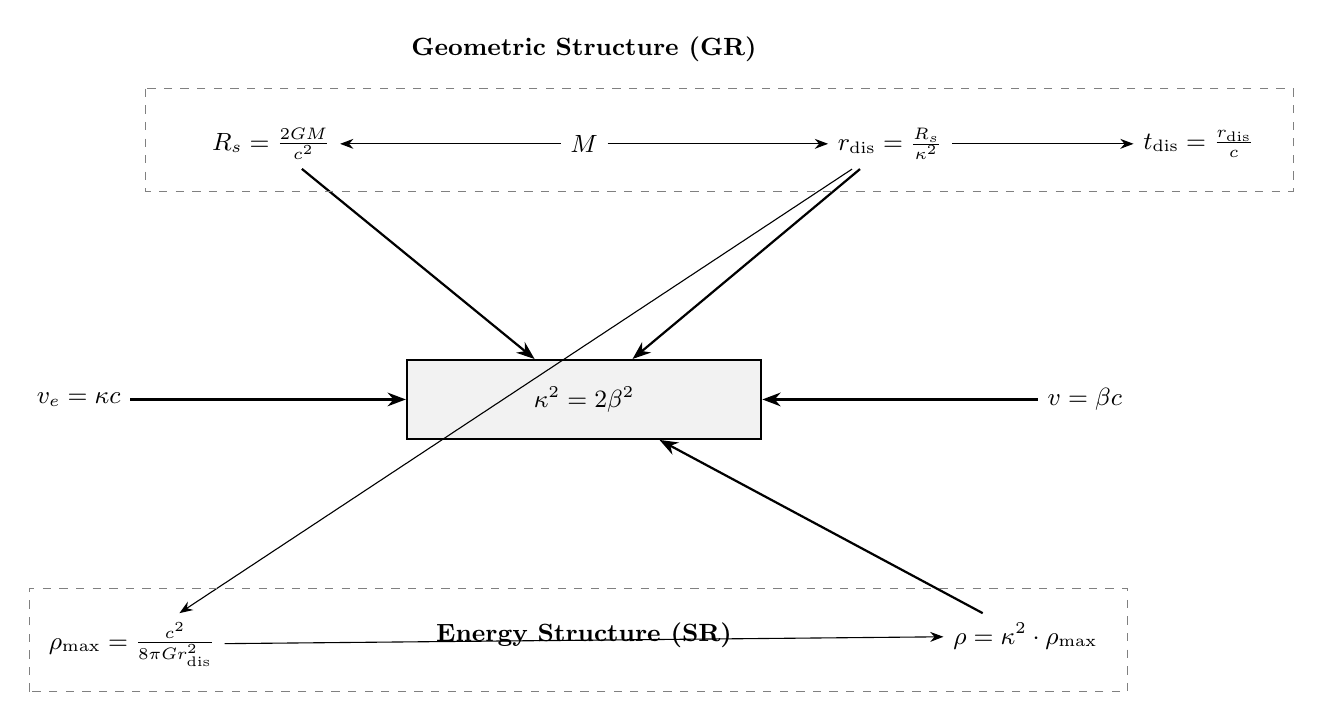
\begin{tikzpicture}[node distance=1.6cm and 2.5cm, every node/.style={font=\small}, >=Stealth]

% Center
\node (center) [draw, thick, rectangle, fill=gray!10, minimum width=4.5cm, minimum height=1cm] {$\kappa^2 = 2\beta^2$};

% Velocities (left and right)
\node (ve) [left=3.5cm of center] {$v_e = \kappa c$};
\node (v) [right=3.5cm of center] {$v = \beta c$};

% Geometry (top)
\node (M) [above=2.5cm of center] {$M$};
\node (Rs) [left=2.8cm of M] {$R_s = \frac{2GM}{c^2}$};
\node (rdis) [right=2.8cm of M] {$r_{\text{dis}} = \frac{R_s}{\kappa^2}$};
\node (tdis) [right=2.3cm of rdis] {$t_{\text{dis}} = \frac{r_{\text{dis}}}{c}$};

% Energy (bottom)
\node (rhomax) [below left=2.2cm and 2.3cm of center] {$\rho_{\text{max}} = \frac{c^2}{8\pi G r_{\text{dis}}^2}$};
\node (rho) [below right=2.2cm and 2.3cm of center] {$\rho = \kappa^2 \cdot \rho_{\text{max}}$};

% Arrows to center
\draw[->, thick] (ve) -- (center);
\draw[->, thick] (v) -- (center);
\draw[->, thick] (Rs) -- (center);
\draw[->, thick] (rdis) -- (center);
\draw[->, thick] (rho) -- (center);

% Geometry arrows
\draw[->] (M) -- (Rs);
\draw[->] (M) -- (rdis);
\draw[->] (rdis) -- (tdis);

% Energy arrows
\draw[->] (rhomax) -- (rho);
\draw[->] (rdis) -- (rhomax);

% Dashed boxed areas
\draw[dashed, gray] ($(Rs)+(-1.6,0.7)$) rectangle ($(tdis)+(1.2,-0.6)$);
\node at ($(M)+(0,1.2)$) {\textbf{Geometric Structure (GR)}};

\draw[dashed, gray] ($(rhomax)+(-1.3,-0.6)$) rectangle ($(rho)+(1.3,0.6)$);
\node at ($(center)+(0,-3.0)$) {\textbf{Energy Structure (SR)}};

\end{tikzpicture}
\end{center}

The result is a structure where \textbf{causality is internal}, \textbf{coherence is enforced},  
and \textbf{dynamics is simply the shifting of balanced configurations} ---  
not the unfolding of arbitrary functions over time.

\subsection{Geometric Prediction of Photon Sphere and ISCO}

\begin{theorem}[Critical Radii Emergence]
In the Will Geometry framework, the critical orbital radii of the photon sphere and innermost stable circular orbit (ISCO) emerge naturally from the geometric equilibrium where $\theta_S = \theta_G$.
\end{theorem}
\begin{proof}
A notable geometric equilibrium occurs at the critical angle 
\begin{equation}
    \theta_S = \theta_G= 54.7356103172^{\circ} \text{ (balance point for photon sphere and ISCO)}
\end{equation}
or approximately $\theta_S = \theta_G \approx 0.9553\,\text{radians}$.

This equilibrium yields the fundamental relation:
\begin{equation}
\kappa^2 + \beta^2 = 1,
\end{equation}
These critical radii emerge spontaneously from the geometry, suggesting inherent spacetime structure without additional assumptions.

\subsubsection{Mathematical Derivation of Critical Points}

Key critical points include:
When:
\begin{itemize}
    \item \(\kappa = \sqrt{\frac{2}{3}} \approx 0.816\) and \(\beta = \frac{1}{\sqrt{3}} \approx 0.577\), corresponding to:
    \[
    r = \frac{R_s}{\kappa^2} =\frac{3}{2}R_s = 1.5R_s \quad \text{(radius of the photon sphere)}.
    \]
    When:
    \item      \( \kappa=\sqrt{\frac{1}{3}}\approx 0.577, \quad \text{and} \quad  \beta = \frac{1}{\sqrt{6}} \approx 0.408\), leading to orbital distance:
    \[
    r = \frac{R_s}{2\beta^2} = \frac{R_s}{2 \cdot \frac{1}{6}} = 3R_s \quad \text{(radius of the innermost stable circular orbit, ISCO)}.
    \]
\end{itemize}

At the critical point where \(\beta = \frac{1}{\sqrt{3}}\) and \(\kappa = \sqrt{\frac{2}{3}}\), the following relationships hold:
\begin{align}
\theta_S &= \theta_G \\
\beta &= T_c \\
\kappa &= L_c \\
\cos(\theta_{G}-\theta_{S}) &= 0 \\
Q_t &= \sqrt{1-Q^2} =\sqrt{1-3\beta^2} = 0 \quad \text{(Instability threshold)}
\end{align}

\begin{tcolorbox}[colback=gray!5,colframe=black!40!black,title=Interpretive Note]
While the radii \(1.5R_s\) (photon sphere) and \(3R_s\) (ISCO) are known from classical General Relativity, their spontaneous emergence from angle equality \(\theta_S = \theta_G\) in our geometric framework is not imposed but arises from internal energy projection symmetries. This correspondence reinforces the internal consistency and explanatory power of Will Geometry.
\end{tcolorbox}

\begin{tcolorbox}[colback=gray!5, colframe=black!80!black, title=Projectional Principle]
\[
\textit{Geometry defines causality before mass, and curvature before gravity.}
\]
\end{tcolorbox}
\end{proof}


\section{Empirical Validation}

\subsection{Energy Reciprocity Validation: GPS Satellite and Earth}

\begin{theorem}[Real-World Energy Reciprocity]
The Energy Reciprocity Law holds precisely for the Earth-GPS satellite system.
\end{theorem}

\begin{proof}
We verify the Energy Reciprocity Law on real orbital data for a GPS satellite and an observer on the Earth's surface, using the following parameters:
\begin{itemize}
\item Gravitational constant: $G = 6.67430 \times 10^{-11}$ m$^3$/kg/s$^2$
\item Speed of light: $c = 2.99792458 \times 10^8$ m/s
\item Mass of Earth: $M_{\text{Earth}} = 5.972 \times 10^{24}$ kg
\item Radius of Earth: $R_{\text{Earth}} = 6.370 \times 10^6$ m
\item Radius of GPS orbit: $r_{\text{GPS}} = 2.6571 \times 10^7$ m
\end{itemize}

The orbital velocity of the GPS satellite is:
\begin{align}
v_{\text{GPS}} &= \sqrt{\frac{GM_{\text{Earth}}}{r_{\text{GPS}}}} \\
&= \sqrt{\frac{6.67430 \times 10^{-11} \times 5.972 \times 10^{24}}{2.6571 \times 10^7}} \\
&= 3873.10090455 \text{ m/s}
\end{align}

Converting to dimensionless parameters:
\begin{align}
\beta_{\text{GPS}} &= \frac{v_{\text{GPS}}}{c} = \frac{3873.10090455}{2.99792458 \times 10^8} =0.0000129192739884 \\
\kappa_{\text{GPS}} &= \sqrt{\frac{2GM_{Earth}}{c^2 r_{GPS}}} =0.0000182706124904 \\
\frac{\kappa_{GPS}^{2}}{\beta_{GPS}^{2}} &=\frac{3.3381528077\times10^{-10}}{1.6690764039\times10^{-10}}=2 \\
Q_{GPS} &=\sqrt{\beta_{GPS}^{2}\ +\kappa_{GPS}^{2}}=0.0000223768389448 \\
Q_{tGPS} &=\sqrt{1-Q_{GPS}^{2}}=\sqrt{1-3\beta_{GPS}^{2}}=0.99999999975
\end{align}
For the Earth's surface:
\begin{align}
\kappa_{\text{Earth}} &= \sqrt{\frac{2GM_{\text{Earth}}}{c^2 R_{\text{Earth}}}} = 0.000037312405944\\
\beta_{\text{Earth}} &= 0 \text{ (at rest)} \\
Q_{Earth} &=\sqrt{\beta_{Earth}^{2}\ +\kappa_{Earth}^{2}}=0.000037312405944 \\
Q_{tEarth} &=\sqrt{1-Q_{Earth}^{2}}=0.999999999304
\end{align}
The time difference between GPS satellite and Earth is:
\[
\Delta Q_{\text{tGPS} \rightarrow \text{Earth}}=(Q_{tGPS}-Q_{tEarth})\cdot 86400  \cdot  10^6  = 38.5124828028 \ \text{micro seconds per day}
\]
This result match empirical data to high precision.

The energy difference from Earth observer to GPS satellite is:
\begin{align}
\Delta E_{\text{Earth} \rightarrow \text{GPS}} &=\left(\kappa_{Earth}^{2}-\beta_{GPS}^{2}\right)= (\kappa^2_{\text{Earth}} - \kappa^2_{\text{GPS}}) + \beta^2_{\text{GPS}} \\
&= (1.3922156373\times10^{-9} - 3.3381528077\times10^{-10}) + 1.6690764039\times10^{-10} \\
&= 1.2253079969\times10^{-9}
\end{align}

The energy difference from GPS satellite to Earth is:
\begin{align}
\Delta E_{\text{GPS} \rightarrow \text{Earth}} &= \left(\beta_{GPS}^{2}-\kappa_{Earth}^{2}\right)=(\kappa^2_{\text{GPS}} - \kappa^2_{\text{Earth}}) - \beta^2_{\text{GPS}} \\
&= (3.3381528077\times10^{-10} - 1.3922156373\times10^{-9}) - 1.6690764039\times10^{-10} \\
&= -1.2253079969\times10^{-9}
\end{align}

Therefore:
\begin{align}
\Delta E_{\text{GPS} \rightarrow \text{Earth}}+\Delta E_{\text{Earth} \rightarrow \text{GPS}}  = -1.2253079969\times10^{-9} + 1.2253079969\times10^{-9} = 0
\end{align}

This confirms the Energy Reciprocity Law to high precision.
\end{proof}

\subsection{Relativistic Precession Validation: Mercury and the Sun}

\begin{theorem}[Relativistic Precession Calculation via Will Geometry]
The relativistic precession of Mercury's orbit matches the classical GR result with high precision, using Will Geometry projection parameters.
\end{theorem}

\begin{proof}
We verify the precession of Mercury's orbit using Will Geometry and compare it to the GR prediction.

\textbf{Input physical parameters:}
\begin{itemize}
\item Gravitational constant: $G = 6.67430 \times 10^{-11}$ m$^3$/kg/s$^2$
\item Speed of light: $c = 2.99792458 \times 10^8$ m/s
\item Mass of the Sun: $M_{\text{Sun}} = 1.98847 \times 10^{30}$ kg
\item Schwarzschild radius of the Sun: $R_{Ssun} = 2.953$ km = $2953$ m
\item Semi-major axis of Mercury: $a_{Merc} = 5.79 \times 10^{10}$ m
\item Eccentricity of Mercury's orbit: $e_{Merc} = 0.2056$
\end{itemize}

\textbf{Dimensionless projection parameters for Mercury:}
\begin{align}
\kappa_{Merc} &= \sqrt{\frac{R_{Ssun}}{a_{Merc}}} = \sqrt{\frac{2953}{5.79 \times 10^{10}}} = 0.000225878693163 \\
\beta_{Merc} &= \sqrt{\frac{R_{Ssun}}{2 a_{Merc}}} = \sqrt{\frac{2953}{2 \times 5.79 \times 10^{10}}} = 0.000159720355661
\end{align}

\textbf{Combined energy projection parameter:}
\begin{align}
Q_{Merc}^{2} &= 3 \beta_{Merc}^{2} = 3 \times (0.000159720355661)^2 = 7.6531776038 \times 10^{-8}
\end{align}

\textbf{Correction factor for the elliptic orbit:}
\begin{align}
\frac{1 - e_{Merc}^{2}}{2\pi} &= \frac{1 - (0.2056)^2}{2 \times 3.14159265359} = \frac{0.9577}{6.28318530718} = 0.152427247197
\end{align}

\textbf{Final Will Geometry precession result:}
\begin{align}
M_{PWILL} &= \frac{3 \beta_{Merc}^{2}}{\frac{1 - e_{Merc}^{2}}{2\pi}} = \frac{7.6531776038 \times 10^{-8}}{0.152427247197} = 5.0208724126 \times 10^{-7}
\end{align}

\textbf{Classical GR prediction for precession:}
\begin{align}
M_{PGR} &= \frac{3\pi R_{Ssun}}{a_{Merc} (1 - e_{Merc}^{2})} = \frac{3 \times 3.14159265359 \times 2953}{5.79 \times 10^{10} \times 0.9577} = 5.0208724126 \times 10^{-7}
\end{align}

\textbf{Relative difference:}
\begin{align}
\frac{M_{PGR} - M_{PWILL}}{M_{PGR}} \times 100 &= \frac{5.0208724126 \times 10^{-7} - 5.0208724126 \times 10^{-7}}{5.0208724126 \times 10^{-7}} \times 100 \\
&= 2.1918652104 \times 10^{-10} \%
\end{align}

This negligible difference is consistent with the numerical precision limits of floating-point arithmetic, confirming that Will Geometry reproduces the observed relativistic precession of Mercury to within machine accuracy.

\end{proof}


\section{Conclusion}

The Will Geometry framework presents a unified mathematical model where Special and General Relativity emerge from the same geometric principles. By focusing on the projectional nature of energy, we have shown that spacetime itself is merely the manifestation of energy's evolution.

From a single postulate—that spacetime is equivalent to energy evolution—we derived all the mathematical apparatus needed to describe gravitational and relativistic phenomena. This unification, showing that energy, time, space, and mass are merely different projections of the same underlying structure.

This approach offers distinct advantages:
\begin{itemize}
\item Conceptual clarity — understanding physics through pure geometry
\item Computational efficiency — reducing complexity by up to 95\%
\item Epistemological hygiene — deriving results from minimal assumptions
\item Philosophical depth — redefining our understanding of time, mass, and causality
\end{itemize}

Will Geometry is not merely a reformulation of existing theories, but a paradigm shift that inverts our fundamental understanding: Energy does not exist within spacetime—spacetime emerges from the evolution of energy.

\begin{tcolorbox}[colback=gray!5, colframe=black!80!black, title=Final Principle]
\textbf{Reality is projectional curvature of energetic flow.}
\end{tcolorbox}
\end{proof}

\section{Epilogue: On the Motivation of This Work}

This work is not the product of formal academic research, institutional funding, or collaboration with established scientific communities. It is the result of personal inquiry, curiosity, and an ongoing attempt to understand the fundamental nature of space, time, and energy from the most elementary and geometric principles.

The motivation behind this framework is rooted in a deep philosophical belief that the structure of the Universe must, at its core, can be described without arbitrary parameters, assumptions, or external mathematical constructs. The ideal theory should not rely on pre-existing formalism but should emerge naturally from the geometry of the Universe itself.

It is important to clarify that I do not consider myself an academic authority, nor do I claim to have discovered any new physical law. I am a self-taught enthusiast, driven not by the desire for recognition but by a personal need to resolve fundamental questions about reality in the simplest possible terms.

Throughout this research, I have maintained a rigorous internal skepticism, questioning every step and assumption. The fact that I have arrived at results equivalent to the standard formulations of Special and General Relativity using only geometric first principles may appear unlikely, even to myself. I fully acknowledge the statistical improbability of such an achievement by an individual without formal academic training.

However, this work is not an attempt to replace or dispute existing physics but rather to reinterpret it from a geometric and philosophical standpoint. Whether this approach holds broader value is irrelevant to its primary purpose — to provide a coherent and intuitive framework that satisfies my own intellectual and philosophical curiosity.

Above all, this document serves as a personal record and reflection of a journey toward understanding, reminding me of the reasons why I chose to embark on this path.


P.S. \textit{This work remains an ongoing exploration, and further developments may reveal deeper connections between geometry, energy, and the fabric of reality.
}

                                                                                                                                                               \subparagraph{\textit{Anton Rize.}}
                                                                                                                                                               
                                                                                                                                                               
\section*{Comparison Table: General Relativity (GR) vs WILL Framework}

\begin{tabularx}{\textwidth}{@{}clXX@{}}
\toprule
\# & Category & \textbf{General Relativity (GR)} & \textbf{WILL Framework} \\
\midrule
1 & Nature of Space and Time & 
Postulated as smooth manifold with metric \( g_{\mu\nu} \) & 
Emerges from projection of energy relations (\( \kappa, \beta \)) \\
\addlinespace

2 & Curvature & 
Defined via \( R_{\mu\nu}, R \); second derivatives of the metric & 
Defined algebraically as \( \kappa^2 = \frac{R_s}{r} \) \\
\addlinespace

3 & Energy and Momentum & 
Encoded in \( T_{\mu\nu} \), requires model of matter & 
Directly given by \( \rho(r) \), \( \rho_{\text{max}}(r) \), and \( p(r) \) \\
\addlinespace

4 & Geometry–Matter Relation & 
\( G_{\mu\nu} = \frac{8\pi G}{c^4} T_{\mu\nu} \); differential equation & 
\( \kappa^2 = \rho / \rho_{\text{max}} \); local proportionality \\
\addlinespace

5 & Singularities & 
Appear when \( \rho \to \infty \), \( g_{00} \to 0 \) & 
Excluded by construction: \( \rho \leq \rho_{\text{max}} \), \( \kappa^2 \leq 1 \) \\
\addlinespace

6 & Gravitational Limitation & 
Via metric behavior and horizons & 
Via geometric constraint \( \kappa \in [0,1] \) \\
\addlinespace

7 & Density Limit & 
Not explicitly defined, requires external input (Planck-scale) & 
Explicitly defined: \( \rho_{\text{max}} = \frac{c^2}{8\pi G r^2} \) \\
\addlinespace

8 & Concept of Time & 
Coordinate-based, embedded in \( g_{00} \); system-dependent & 
Physical: \( \beta \) as projection of energy onto temporal axis \\
\addlinespace

9 & Dynamics & 
Via time derivatives and Lagrangians & 
Via change in energy proportions; no differential equations \\
\addlinespace

10 & Formalism & 
Geometry, tensors, 2nd-order derivatives & 
Energy projections, circular geometry, algebraic closure \\
\addlinespace

11 & Intuitiveness & 
Low; relies on abstract and heavy formalism & 
High; built from observable and intrinsic relations \\
\addlinespace

12 & Observational Fit & 
Confirmed (with dark matter/energy assumptions) & 
Consistent; explains phenomena without "dark entities" \\
\bottomrule
\end{tabularx}








\section{Key Equations Reference}

This section serves as a convenient reference for the core equations and relationships of the Energy Geometry framework.

\subsection{Fundamental Parameters}

\begin{align}
   \textbf{Kinematic projection} \quad  \beta &=  \frac{v}{c} = \sqrt{\frac{R_s}{2r_{dis}}} = \sqrt{\frac{Gm_0}{r_{dis}c^2}} = \cos\left(\theta_S\right), \quad \text{(Orbital velocity)} \\
 \textbf{Potential projection} \quad  \kappa &= \frac{v_e}{c} = \sqrt{\frac{R_s}{r_{dis}}} = \sqrt{\frac{2Gm_0}{r_{dis}c^2}} = \sqrt{\frac{\rho}{\rho_{max}}}= \sin\left(\theta_G\right), \quad \text{(Escape velocity)}
\end{align}

\subsection{Core Relationships}

\begin{align}
    \kappa^2 &= 2\beta^2 \quad \text{(Fundamental projection ratio)} \\
    \frac{\kappa}{\beta} &= \sqrt{2} \\
    \kappa^2 + \beta^2 &= 3\beta^2 = \frac{3}{2}\kappa^2 = \frac{3R_s}{2r_{dis}} \\
    \frac{r_{dis}}{R_s} &= \frac{1}{\kappa^2} = \frac{1}{2\beta^2}
\end{align}

\subsection{Mass, Energy and Distance}

\begin{align}
    m_0 &= \frac{\kappa^2 c^2 r_{dis}}{2G} = \frac{R_s c^2}{2G} \quad \text{(mass of the system or object)} \\
    r_{dis} &= \frac{R_s}{\kappa^2} = \frac{2Gm_0}{\kappa^2 c^2}  \quad \text{(radial distance)}\\
    t_{dis} &= \frac{r_{dis}}{c}  \quad \text{(temporal distance)}\\
    R_s &= \frac{2Gm_0}{c^2}=\kappa^2 r_{dis} \quad \text{(critical radial distance)} \\
    \frac{m_0}{r_{\text{dis}}} \cdot \frac{l_P}{m_P} &= \beta^2 \quad \text{(Universal mass-to-distance ratio)}
\end{align}

\subsection{Energy Density and Pressure}

\begin{align}
    \rho &= \frac{\kappa^2 c^2}{8\pi G r_{dis}^2} = \kappa^2 \cdot \rho_{max} \\
    \rho_{max} &= \frac{c^2}{8\pi G r_{dis}^2} \quad \text{(Critical energy density)} \\
    P(r_{dis}) &= - \frac{c^2}{8\pi G} \cdot \frac{1}{r_{dis}} \cdot \frac{d\kappa^2}{dr_{dis}} \quad \text{(Pressure)}
\end{align}

\subsection{Contraction and Dilation Factors}

\begin{align}
    L_c &= \sin\left(\theta_S\right) = \sqrt{1 - \beta^2} \quad \text{(Relativistic length contraction)} \\
    T_c &= \cos\left(\theta_G\right) = \sqrt{1 - \kappa^2} \quad \text{(Gravitational time contraction)} \\
    T_d &= \frac{1}{L_c} = \frac{1}{\sqrt{1-\beta^2}} \quad \text{(Relativistic time dilation)} \\
    L_d &= \frac{1}{T_c} = \frac{1}{\sqrt{1-\kappa^2}} \quad \text{(Gravitational length dilation)}
\end{align}

\subsection{Combined Energy Parameter $Q$:}
The total energy projection parameter unifies both aspects:

\begin{align}
    Q &=\sqrt{\kappa^2 + \beta^2}  \\
    Q^{2}&= 3\beta^2 = \frac{3}{2}\kappa^2 = \frac{3R_s}{2r_{dis}} \\
    Q_t &= \sqrt{1-Q^2} = \sqrt{1-\kappa^2-\beta^2} = \sqrt{1-3\beta^2} = \sqrt{1-\frac{3}{2}\kappa^2} \\
    Q_r &= \frac{1}{Q_t}
\end{align}

These describe the combined effects of relativity and gravity.

\subsection{Circle Equations}

\begin{align}
    2\beta^2 + T_c^2 &= 1 \\
    \frac{\kappa^2}{2} + L_c^2 &= 1 \\
    2\cos^2(\theta_S) + \cos^2(\theta_G) &= 1 \\
    2\beta^2 + (1-\kappa^2) &= 1
\end{align}

\subsection{Unified Field Equation}

\begin{align}
    \frac{d}{dr_{dis}}(\kappa^2 \cdot r_{dis}) &= \frac{8\pi G}{c^2} r^2_{dis} \cdot \rho(r_{dis}) \\
    \frac{R_s}{r_{dis}} &= \frac{\rho}{\rho_{max}} = \kappa^2
\end{align}

\subsection{Fundamental Will Invariant}

\begin{align}
    W_{ill} &= \frac{E \cdot T^2}{M \cdot L^2} = \frac{L_d\,E_0\,T_c\,t_{dis}^{2}}{T_d\,m_0\,L_c\,r_{dis}^{2}}= \frac{\frac{1}{\sqrt{1-\kappa^{2}}}m_{0}c^{2}\cdot\sqrt{1-\kappa^{2}}\left(\frac{2Gm_{0}}{\kappa^{2}c^{3}}\right)^{2}}{\frac{1}{\sqrt{1-\beta^{2}}}m_{0}\cdot\sqrt{1-\beta^{2}}\left(\frac{2Gm_{0}}{\kappa^{2}c^{2}}\right)^{2}}=1 \\
\end{align}

\subsection{Special Points}

\begin{align}
    \text{Photon Sphere:} \quad r &= \frac{3}{2}R_s \quad \text{where} \quad \kappa = \sqrt{\frac{2}{3}} \approx 0.816, \beta = \frac{1}{\sqrt{3}} \approx 0.577 \\
    \text{ISCO:} \quad r &= 3R_s \quad \text{where} \quad \beta = \frac{1}{\sqrt{6}} \approx 0.408
\end{align}

At the critical point where $\theta_S = \theta_G = 54.7356103172^{\circ}$:
\begin{align}
    \kappa^2 + \beta^2 &= 1 \\
    \beta &= T_c \\
    \kappa &= L_c \\
    Q_t &= \sqrt{1-3\beta^2} = 0 \quad \text{(Instability threshold)}
\end{align}


\end{document}